\documentclass[12pt,letterpaper]{article}

\usepackage{amsmath, amsthm}
\usepackage{graphicx,hyperref}
\usepackage{microtype, parskip}
\usepackage{natbib}
\usepackage{lineno}
\usepackage[font=small]{caption}
\usepackage{subcaption, multirow, morefloats}
\usepackage{subcaption, wrapfig}
\usepackage{rotating}
\usepackage{titlesec}
\usepackage[nottoc,numbib]{tocbibind}
\usepackage{authblk, attrib, fullpage}
\usepackage{lineno}

\frenchspacing

\captionsetup[subfigure]{position = top, labelfont = bf, textfont = normalfont, singlelinecheck = off, justification = raggedright}

\renewcommand{\section}[1]{%
\bigskip
\begin{center}
\begin{Large}
\normalfont\scshape #1
\medskip
\end{Large}
\end{center}}

\renewcommand{\subsection}[1]{%
\bigskip
\begin{center}
\begin{large}
\normalfont\itshape #1
\end{large}
\end{center}}

\renewcommand{\subsubsection}[1]{%
\vspace{2ex}
\noindent
\textit{#1.}---}

\renewcommand{\tableofcontents}{}

\bibpunct{(}{)}{;}{a}{}{,}  % this is a citation format command for natbib

\title{How cryptic is cryptic diversity? Machine learning approaches to classifying morphological variation in the Pacific Pond Turtle (\textit{Emys marmorata})}
%\title{Supervised learning approaches to quantifying cryptic diversity: picking amongst taxonomic hypotheses of Pacific Pond Turtle (\textit{Emys marmorata})}
\author[1]{Peter D Smits}%\thanks{psmits@uchicago.edu}}
\author[1,2]{Kenneth D Angielczyk}%\thanks{kangielczyk@fieldmuseum.org}}
\author[3]{James F Parham}%\thanks{jparham@fullerton.edu}}
\author[4]{Bryan Stuart}%\thanks{bryan.stuart@naturalsciences.org}}
\affil[1]{Committee on Evolutionary Biology, University of Chicago}
\affil[2]{Integrative Research Center, Field Museum of Natural History}
\affil[3]{Department of Geological Sciences, California State University -- Fullerton}
\affil[4]{Section of Research and Collections, North Carolina Museum of Sciences}


\begin{document}
\maketitle
\noindent{\textbf{Corresponding author:} Peter D Smits, Committee on Evolutionary Biology, University of Chicago, 1025 E. 57th Street, Culver Hall 402, Chicago, IL, 60637, USA; E-mail: \href{mailto:psmits@uchicago.edu}{psmits@uchicago.edu}}

\linenumbers
\modulolinenumbers[2]

\begin{abstract}
\end{abstract}

\section{Introduction}


\section{Materials and Methods}
\subsection{Specimens, sampling, morphometrics}
Three different landmark-based morphometric datasets describing plastron variation were assembled for this analysis: specimens from seven distinct emydine species, \textit{T. scripta} specimens from both subspecies, and \textit{E. marmorata} specimens from across its geographic range. We chose to focus on adults because significant changes in plastron shape occur over the course of ontogeny in \textit{E. marmorata} and other emydines \citep{Angielczyk2013a}.
% three turtle datasets
%   seven species
%   Trachemys species
%   Emys complex
% 26 landmarks

The first dataset is a compilation of 101 specimens of \textit{T. scripta}: 51 specimens of \textit{T. scripta scripta} and 50 specimens of \textit{T. scripta scripta}. These landmark data are new to this study. 

The second dataset, we analyzed 578 total specimens from the following species: \textit{Emys blandigii}, \textit{Terrapene coahuila}, \textit{Clemmys guttata}, \textit{Glyptemys insculpta}, \textit{Glyptemys muhlenbergii}, \textit{Emys orbicularis}, and \textit{Terrapene ornata}. Like the first data set, these specimens are a subset of those used in \citet{Angielczyk2011} and \citet{Angielczyk2013a}.

The final dataset dataset included 354 adult \textit{E. marmorata} museum specimens; a subset of those included in \citet{Angielczyk2007}, \citet{Angielczyk2011}, and \citet{Angielczyk2013a}. We assigned a classification to each specimen for the different binning schemes based on geographic occurrence data recorded in museum collection archives. When precise latitude and longitude information were not available we estimated them from locality information. Because \citet{Spinks2005}, \citet{Spinks2010}, and \citet{Spinks2014} did not use vouchered specimens we were not able to directly sample the individuals in their studies. Therefore our specimen classifications were based solely on the geographic information, not explicit assignment using molecular data. Because the exact barriers between different biogeographic regions are unknown and unclear, we represented some hypothesis with two schemes for a total of six different schemes. These schemes differed based on where geographic boundaries were assigned. This changes the classification of certain individuals near the boundaries between groups, providing a test of the robustness of the classification schemes. Sex information was only know for a subset of the total dataset and was not included as a predictor of classification. Sex information was used to determine if observations cluster by sex or not. The scheme names are as follows: Mito 1 and 2 correspond to \citet{Spinks2005}, Mito 3 corresponds to \citet{Spinks2010}, Morph 1 and Morph 2 correspond to \citet{Holland1992}, and Nuclear corresponds to \citet{Spinks2014}. 


\begin{figure}[h]
  \centering
  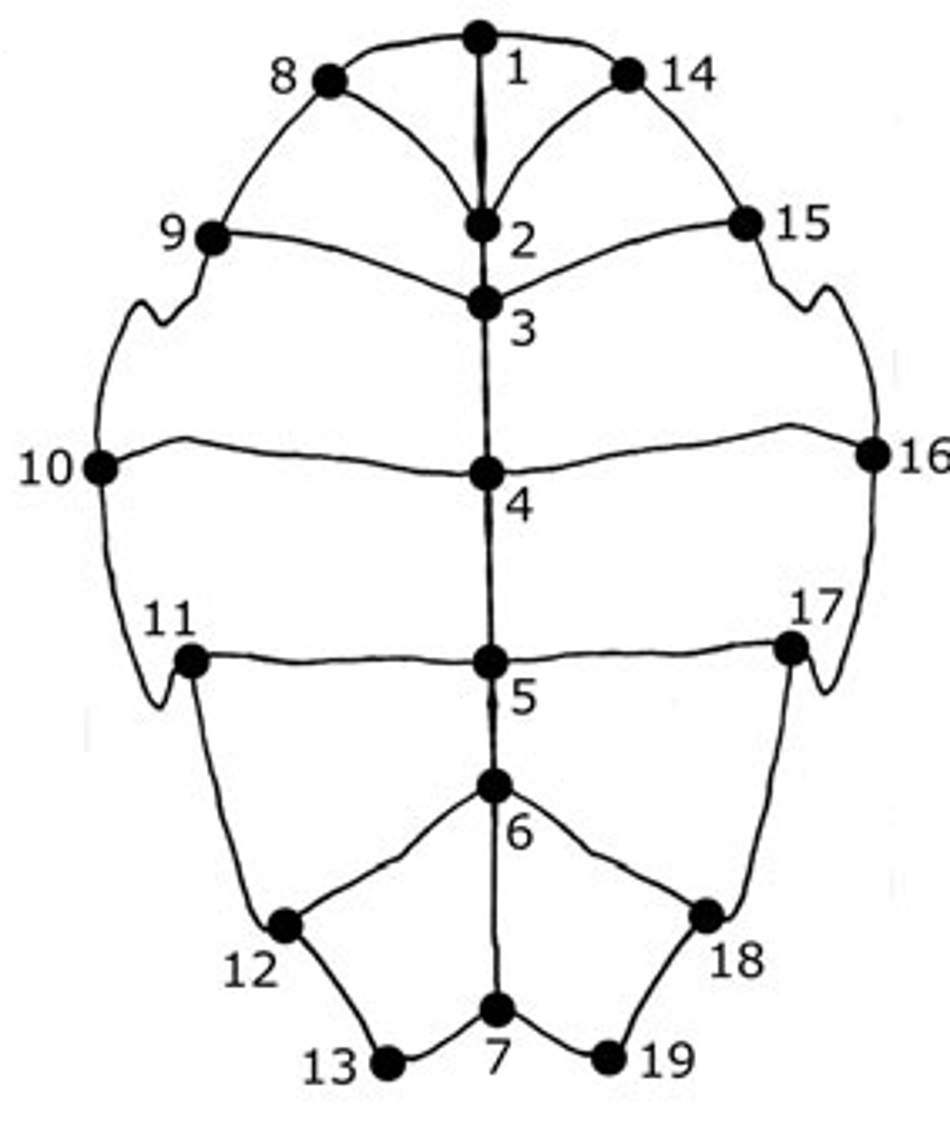
\includegraphics[height = 0.5\textheight, width = \textwidth, keepaspectratio = true]{figure/plastra}
  \caption{Depiction of general plastral shape of \textit{E. marmorata} and position of the 19 landmark used in this study. Anterior is towards the top of the figure.}
  \label{fig:plastra}
\end{figure}


Following previous work on plastron shape \citep{Angielczyk2007,Angielczyk2011,Angielczyk2013a}, we used TpsDig 2.04 \citep{Rohlf2005} to digitize 19 landmarks (Fig. \ref{fig:plastra}). Seventeen of the landmarks are at the endpoints or intersection of the keratinous plastral scutes that cover the plastron. Twelve of the landmarks were symmetrical across the axis of symmetry. Because damage prevented the digitization of all the symmetric landmarks in some specimens, we reflected landmarks across the axis of symmetry (i.e. midline) prior to analysis and used the average position of each symmetrical pair. In cases where damage or incompleteness prevented symmetric landmarks from being determined, we used only the single member of the pair. We conducted all subsequent analyses on the resulting ``half'' plastra. We superimposed the plastral landmark configurations using generalized Procrustes analysis \citep{Dryden1998a}, after which, we calculated the principal components (PC) of shape using the \texttt{shapes} package for R \citep{2015,Dryden2013}.


\subsection{Biasing effects}
% digitization
We estimated the possible effect of digitization error CITATIONS on our results by comparing within (replicated) specimen Procrustes distances to the distances between classification scheme centroids. 10 randomly selected specimen both for this study and an additional four times. These 50 landmark configurations were then Procrustes superimposed. A range of four Procrustes distances were then calculated as the average of the pairwise distances between each of the replicate configurations. These distances were then compared to the average pairwise Procrustes distance between the class centroids for each classification schemes of \textit{E. marmorata} being analyzed.

% sex
% permutation test
%   is the distance between sex means bigger than expected by random?


\subsection{Supervised learning approaches}
% predictors/features/covariates
%   1:25 PCs
%   size
%   size X PC1
% analogy to PCA regression
The maximum set of possible predictors or features used for any model are the first 25 principal components (PCs), scaled centroid size, and the interaction between scaled centroid size and PC 1. Size and the interaction between size and PC 1 were included as predictors in order to account for a possible interaction between size and shape over the duration of an individual as well as potential size differences between classes, even if this is unlikely \citep{Seeliger1945,Holland1992}. We say ``maximum set'' because the best or selected models based on 5-fold cross-validation does need not to, nor will they likely, include all predictors possible (see below).

This approach is in many ways analogous to PCA regresion. PCA regression takes advantage of two aspects of PCA for improving regression fit \citep{Hastie2009}. Because the PCs of shape are by definition orthagonal, allowing them to easily as independent predictors or features of class membership without fear of colinearity.

% auc of roc as performance measure
%   relationship between false positive rate and true positive rate
%   varies between 0.5 and 1 (random -- perfect)
%   better performance than accuracy when groups unbalanced
In classification studies, such as this one, a common metric of performance is the receiver operating characteristic (ROC) which is the relationship between the false and true positive rates \citep{Hastie2009}. The area under the ROC curce (AUC) is then the derived estimate of the model performance; AUC ranges from 0.5 to 1 which corresponding to performance similar to random guesses and perfect classificationrates, respectively \citep{Hastie2009}. Both ROC and AUC are preferrable to simple classificaiton accuracy when class membership is unbalanced, as it is in these analyses \citep{Hastie2009}. The standard ROC and AUC calculations are defined only for binary classifications. To generalize this approach for mulitple response classes, we used an all-against-one strategy where the model AUC is the average of the AUC values from the multiple binary comparisons of one class compared to all others \citep{Hand2001}. 


% training and testing paradigm
%   training dataset
%     for multiple models with between 3 and 28 predictors
%     5-fold cross validation of each model
%     best model had greatest mean AUC value
%     selected model is most parsimonious model within 1 SD of ROC of best model
%   testing dataset
%     estimate class of out-of-sample testing dataset
%     compare average AUC across models for each scheme
% caret package for R
We adopted a training and testing paradigm for selecting parsimonious models and estimating their overall error rates \citep{Hastie2009,Kuhn2013}. Within-sample model performance is inherently biased upwards, so model evaluation requires overcoming this bias. With very large sample sizes, as in this study, part of the sample can be used as the ``training set'' and the remainder acts as the ``testing set.'' In this approach, following all cleaning and vetting, the data is split into a training dataset and a testing dataset. The former is used for fitting the model where as the later is used for measuring model performance, a process called model generalization. In this analysis, we used 80\% of samples as the training set while the remaining 20\% were used as the testing set. 

For a given supervised learning method, we compared the fit of 27 models as the average AUC from 10 rounds of 5-fold cross-validation. Cross-validation is an approach for estimating the average out-of-sample predictive error of a model by simulating out-of-sample data from the training data itself \citep{Hastie2009}. In a single round of \(k\)-fold cross-validation, the training data is divided into \(k\) blocks where the model is fit to \(k - 1\) blocks and the values of the \(k\)th block are predicted; this is then repeated for all combinations of blocks. Within each round, the predictive performance metrics is averaged across all folds. Finally, the predictive performance metric is the averaged across all rounds of \(k\)-fold cross-validation. This process was implemented using the R package \texttt{caret} CITATION.

For a given supervised learning method, the ``best'' trained model is that the highest mean AUC as estimated from 5-fold cross-validation. The selected or final model, however, is the next most parsimonious model that is within one standard error of the best model; this is a variant on the ``one-standard error'' rule from \citet{Hastie2009}.

% use multiple methods
%   multinomial logistic regression (nnet)
%   linear discriminate analysis (MASS)
%   penalized discriminate analysis (mda)
%   neural network (nnet)
%   random forest (randomForest)
% each method has different assumptions and treat data differently
%   all assume that predictors have additive effect (e.g. independent)
The supervised learning methods used here were multinomial logistic regression (MLR), linear discrminiate analysis (LDA), penalized discriminate analysis (PDA), single-hidden-layer neutral network (NN), and random forests (RF). Each of these methods makes different assumptions, treat data differently, and can produce very different classification results \citep{Hastie2009}. The common assumption of all of these methods is that the predictors or features are independent and/or have additive effects on prediction \citep{Hastie2009}.



\section{Results}

\subsection{Biasing effects}

\subsection{Supervised learning}

\begin{figure}[ht]
  \centering
  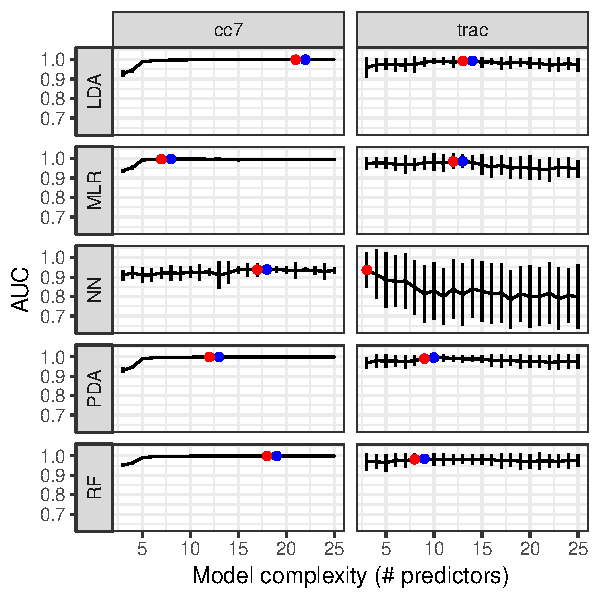
\includegraphics[height = \textheight, width = \textwidth, keepaspectratio = true]{figure/other_model_sel}
  \caption{CAPTION}
  \label{fig:other_sel}
\end{figure}

\begin{figure}[ht]
  \centering
  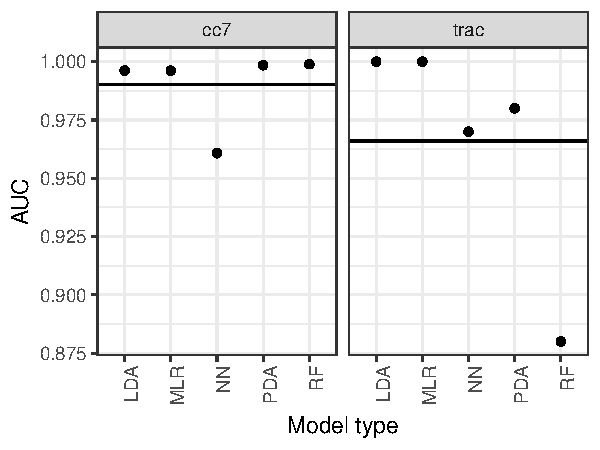
\includegraphics[height = \textheight, width = \textwidth, keepaspectratio = true]{figure/other_oos_sel}
  \caption{CAPTION}
  \label{fig:other_oos}
\end{figure}

\begin{figure}[ht]
  \centering
  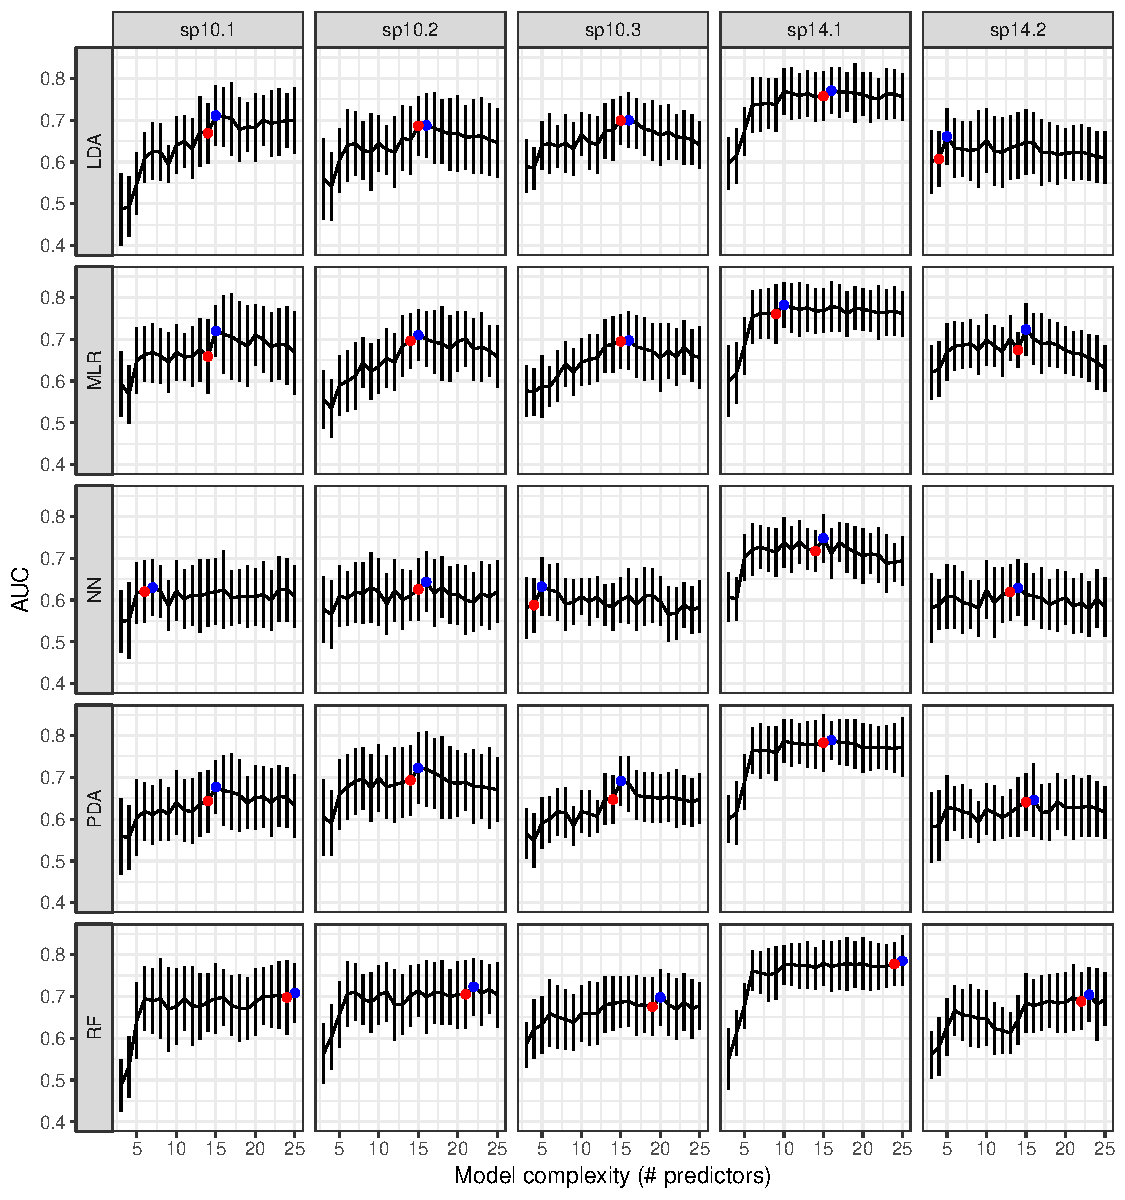
\includegraphics[height = \textheight, width = \textwidth, keepaspectratio = true]{figure/emys_model_sel}
  \caption{CAPTION}
  \label{fig:emys_sel}
\end{figure}

\begin{figure}[ht]
  \centering
  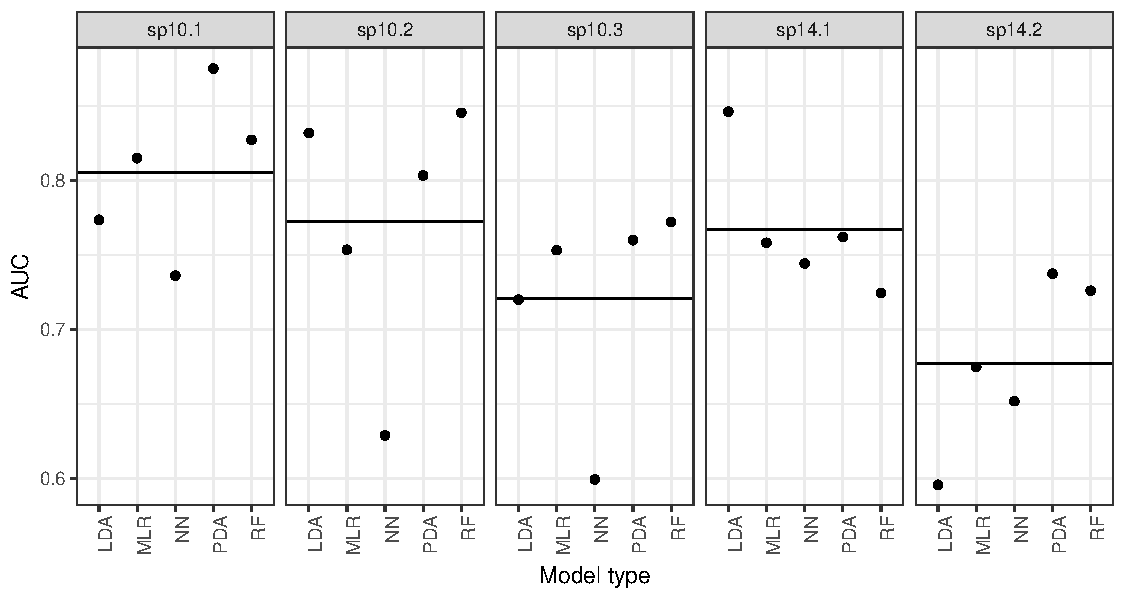
\includegraphics[height = \textheight, width = \textwidth, keepaspectratio = true]{figure/emys_oos_sel}
  \caption{CAPTION}
  \label{fig:emys_oos}
\end{figure}


\section{Discussion}



\section*{Acknowledgements}
Data collection for this project was supported in part by NSF DBI-0306158 (to KDA). G. Miller assisted with data collection and her participation in this research was supported by NSF REU DBI-0353797 (to R. Mooi of CAS). For access to emydine specimens, we thank: J. Vindum and R. Drewes (CAS); A. Resetar (FMNH); R. Feeney (LACM); C. Austin (LSUMNS); S. Sweet (MSE); J.McGuire and C. Conroy (MVZ); A. Wynn (NMNH); P. Collins (SBMNH); B. Hollingsworth (SDMNH); P. Holroyd (UCMP). We are grateful for S. Sweet for field assistance and the California Department of Fish and Game for permits.

\bibliographystyle{abbrvnat}
\bibliography{turtle,packages}

\end{document}
